\chapter{Introduction}
\begin{figure}
	\centering
	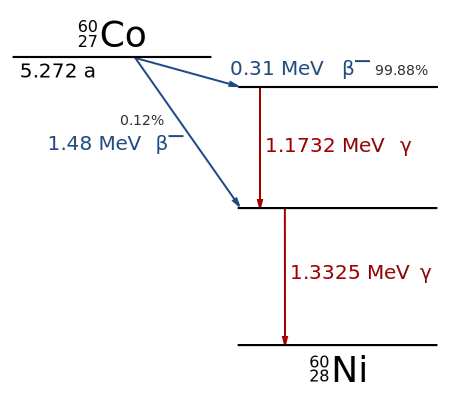
\includegraphics[width=.7\textwidth]{./img/co60_decay.pdf}
	\caption*{Source}
	\caption[The decay cascade of \ce{^{60}Co}]{\textbf{The decay cascade of \ce{^{60}Co}} After decaying from a 5+ spin state to a 4+ spin state of \ce{^{60}Ni} by beta decay with a probability of \num{99.88}\%, two gamma rays of energies \SI{1.17}{\MeV} and \SI{1.33}{\MeV} are emitted, each inhibting a spin of 2+.}
	\label{fig:co60_cascade}
\end{figure}
When the nucleus emits two gamma rays in a cascade, as shown in \autoref{fig:co60_cascade}, the spatial angular distribution of the second particle with respect to the first particle's direction of travel is anisotropic.
In particular, by detecting two particles of a cascade simultaneously, the equal engagement of states is removed, resulting in an anisotropy of the second particle.
The relative probability of the gamma particle's emission at an angle $\theta$ relative to the first photon is denoted as $W(\theta)$.
Normalizing this differential cross-section at $\theta=\SI{90}{\degree}$ yields the correlation function

\begin{equation*}
	K(\theta) &= 1 + \sum_{k}^{k_\text{max}}a_{2k}\cdot\cos^{2k}{\theta}.
\end{equation*}

The series terminates at $k_\text{max}=\min(I, L_1, L_2)=2$, where $I, L_1, L_2$ denote the nuclear spin after the first gamma emission and the angular momenta of both gamma rays respectively.
This results in the correlation function

\begin{equation}\label{eq:corr_func}
	K(\theta) &= 1 + a_2\cos^{2}{\theta} + a_4\cos^{4}{\theta},
\end{equation}
while only pure multipole orders (quadrupoles) are assumed.
